\subsection{Überwachungssysteme}
\label{monitor}
Überwachungssysteme wurden für den Zweck entwickelt den Status von verschiedenen Objekten meist über das Netwerk zu überwachen und im Falle einer Statusänderung diese Information an die zugewiesenen Kontaktpersonen weiterleitet.

Bei diesen Objekten kann es sich um viele verschiedene Komponenten handeln.
Generell unterscheidet man zwischen der Überwachung ermöglichten zu Grunde liegenden Hardware den so genannten Hosts und den auf diesen Hardwarekomponenten aufsitzenden Diensten auch Services genannt.

Unter Hosts fallen nicht nur Server bzw. Computer, sondern auch Switches, Router oder auch explizite / dedizierte / (nur für den/einen Zweck der Überwachung halt) Überwachungshardware wie Sensoren für Temperatur, Luftfeuchtigkeit oder Rauchmelder.
Die Services dieser Hosts weichen je nach Art der Hosts stark voneinander ab.
Auf einem Server kann als Service ein Webserver im Betrieb sein, dessen Funktionalität sich simpel über einen Aufruf einer Webseite überprüfen lässt.
Bei einem Switch können beispielsweise als Service die Übertragungsrate, der Paketverlust oder der Portzustand überwacht werden.

Sehr wichtig ist bei einem Überwachungssystem die Gewichtung der erhaltenen Überwachungsinformationen.


%\begin{center}
%was ist wichtig was nicht, Gewichtung, Klassifizierung, Organisationsstrategie
%Host,Services erklären
%\end{center}

Vor der Einführung eines Überwachungssystems muss sich mit den folgenden Punkten auseinandergesetzt werden.

\subsubsection{Ressourcenbelastung}
Die Einführung einer Überwachungssoftware bringt bei größeren Serverlandschaften eine nicht zu verachtende Netzwerk- und Prozessorbelastung mit sich.
Dabei gilt es die anfallende Belastung durch zwei unterschiedliche Arten der Überwachung zu unterscheiden:

\paragraph{Lokale / Zentrale Bearbeitung}
Die Durchführung der Überprüfungen findet durch einen zentralen Überwachungsserver statt, der die Informationen über die einzelnen Hosts und Services über das Netzwerk abfragt.
Diese Methode ist in der Regel vorzuziehen, da hierbei die zu überwachenden Geräte weniger belastet werden und die Konfiguration der einzelnen Kontrollschritte zentral möglich / realisierbar ist.

\paragraph{Entfernte / Ausgelagerte Bearbeitung}
Bei einer sehr hohen Anzahl von zu überwachenden Objekten ist eine zentralisierte Ausführung nicht mehr von einem einzelnen Server tragbar.
In diesem Fall ist das Überwachungssystem darauf angewiesen, dass die einzelnen Hosts die kontrollierenden Überprüfungen selbständig durchführen und deren Ergebnisse an den Überwachungsserver weiterzuleiten.

%Nagios bietet zusätzlich noch eine weitere, dritte Möglichkeit durch das \textit{Distributed Monitoring} (Verteilte Überwachung) an, siehe Kapitel \ref{dismoni}.

\subsubsection{Netzwerkstruktur und Abhängigkeiten}
Die Überwachung von Hosts und Services über das Netzwerk erzeugt normalerweise immer zusätzlichen \gls{IP}-Traffic.
Das bedeutet, dass jede Überquerung weiterer Netzwerkknoten, die zwischen dem Überwachungsserver und den zu überwachenden Geräten liegen, eine weitere Belastung für das Netzwerk bedeutet, sowie eine Abhängigkeit zwischen Host und Server einführt.

\begin{figure}[ht]
	\centering
	   \fbox{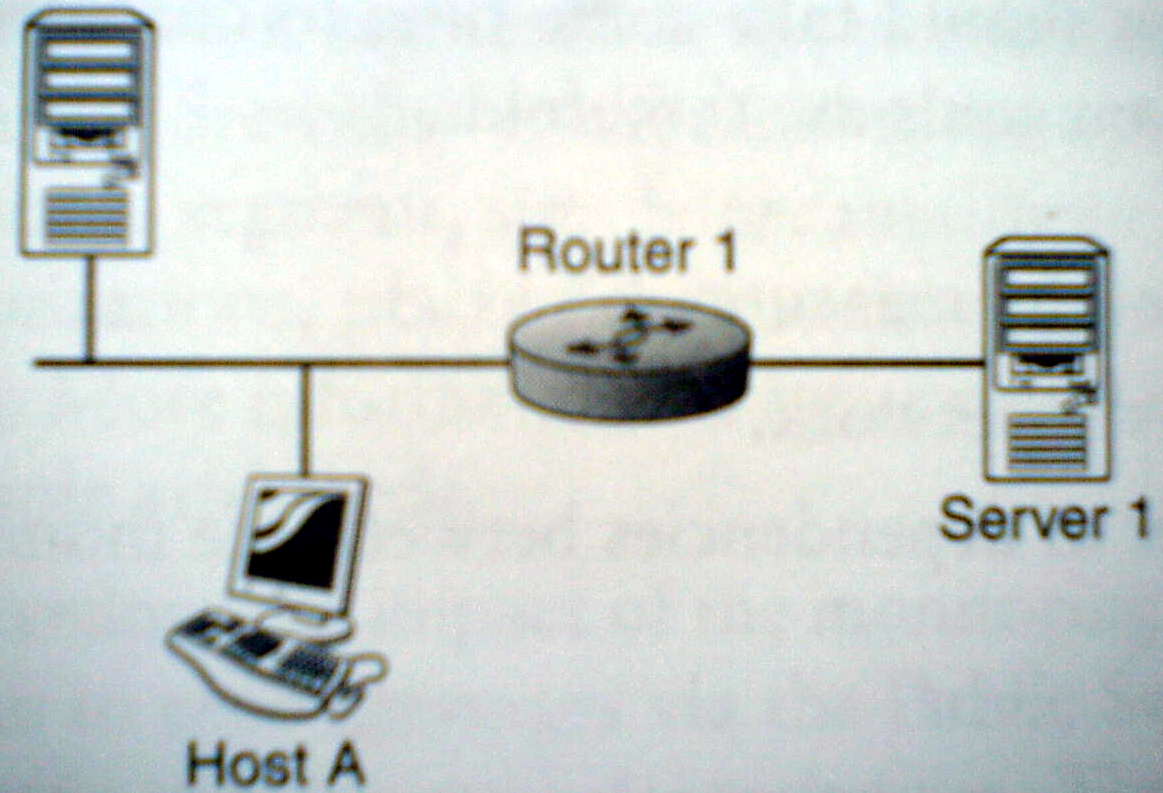
\includegraphics[width=0.38\textwidth]{bilder/dependent.png}}
	   %\fbox{Quelle: \cite{Jose07} S. 5}
		\caption[Zusätzliche Netzwerkabhängigkeit und Netzwerkbelastung]{Zusätzliche Netzwerkabhängigkeit und Netzwerkbelastung\protect\footnote}
		\label{depend}
\end{figure}
\footnotetext{Quelle: \cite{Jose07} S. 5}
\newpage
In der Abbildung \ref{depend} erzeugt der Router 1 die zuvor beschriebene zusätzliche Netzwerkabhängigkeit und Netzwerkbelastung, da der Server 1 bei einem Ausfall des Routers nicht mehr durch den Überwachungsserver erreichbar ist und jede Überprüfung, die vom Überwachungsserver gesendet wird den Router mit dem Routing der Pakete belastet.

Deshalb gilt es laut \cite{Jose07} S. 5 folgende zwei Punkte beim Erstellen eines Überwachungssystems zu beachten:

\paragraph{Überwachungsredundanzen vermeiden}
Redundante Überwachung entsteht dadurch, dass der gleiche Service durch zwei Arten mit unterschiedlichen Tiefen / Tiefgang geprüft wird.
Ein einfaches Beispiel ist die Überwachung eines Webservers auf dem Standardport 80.
Eine Überwachungsmethode ist es diesen Port abzufragen und die entsprechende Rückantwort des Servers auszuwerten.
Soll die auf dem Webserver laufende Webseite überwacht werden, kann die jeweilige Webseite über die Adresse nach einem bestimmten Inhalt untersucht werden.

In beiden Fällen wird getestet, ob der Webserver über das Netzwerk ansprechbar ist, jedoch sagt der zweite Test zusätzlich noch aus, dass die Webseite korrekt angezeigt wird, somit wäre der erste Test überflüssig.
Jedoch muss zuvor abgewogen werden, ob eine redundante Überwachung nicht sogar hilfreich bei der Ermittlung der Fehlerursache ist.
Wenn im oberen Beispiel der Inhalt der überwachten Webseite verändert wird, ist dies nur aus dem zweiten Test ersichtlich.
%, dass der Webserver einwandfrei funktioniert.

\paragraph{Minimale Netzwerkbelastung}
Um bereits stark belastete Netzwerkpunkte zu entlasten, bietet es sich an die Frequenz mit der die Test über das Netzwerk gesendet werden zu verringern.
Die Aufstellung des Überwachungsservers ist dadurch gerade bei größeren Serverlandschaften sehr wichtig, da durch eine effiziente Platzierung womögliche Flaschenhälse / Engstellen in Form von veralteten Switches oder ähnlichem vermieden werden können.

\subsubsection{Sicherheitsaspekte}
Um erweiterte Statusinformationen über einen Prozess oder über die Arbeitsspeicherauslastung auszulesen ist (meistens) zusätzliche Software auf den Hosts nötig.
Diese Software benötigt einen zusätzlichen geöffneten Port auf dem zu überwachendem Rechner, die einen neuen Angriffspunkt für Angreifer darstellen kann.
Außerdem erhält der Überwachungsserver Ausführungsrechte auf dem Client, so dass eine weitere potentielle Sicherheitslücke in einem (vermeintlich) zuvor sicherem System entsteht.
Jeder, der die Kontrolle über den Überwachungsserver besitzt oder sich als solcher ausgibt, kontrolliert somit gleichzeitig alle anderen überwachten Hosts.

Um dies zu verhindern gibt es verschiedene Ansätze.
Als ersten Ansatz sollte der Port durch den der Überwachungsserver mit dem Host kommuniziert vom Standardwert abweichen, damit nicht sofort erkennbar ist, dass sich eine (womöglich) angreifbare Überwachungssoftware auf dem Rechner befindet.\label{changeport}
Damit die über diesen Port versendeten Informationen nicht für Dritte zugänglich sind, bietet es sich an die auszutauschende Informationen mit einem Algorithmus zu verschlüsseln.
Durch den Einsatz eines Verschlüsselungsalgorithmus werden die Informationen nicht mehr im Klartext ausgetauscht, sondern
Da die Möglichkeit einer Verschlüsselung der Datenübertragung nicht von jeder Überwachungssoftware angeboten wird, gilt diese Option als Auswahlkriterium in der späteren Umsetzung bzw. im produktivem Betrieb. (Verweis auf Windows Agenten Übersicht?)

Des weiteren sollte die Erlaubnis der Abfrage der Überwachungsinformationen anhand der \gls{IP}-Adresse eingeschränkt werden, so dass der Client nur Anfragen des Überwachungsservers akzeptiert.
Durch diese Einschränkung kann vermieden werden, dass sensible Informationen aus den Antworten an unberechtigte Dritte übermittelt werden oder ein Denial of Service-Angriff (\gls{DoS}) durch eine übermäßig hohe Anzahl an Anfragen an den Client gesendet wird, um eine Überlastung des Servers zu erreichen und diesen somit arbeitsunfähig zu machen.

%\begin{itemize}
%\item Verschlüsselung der Informationen, die zwischen dem Server und dem Host hin- und hergesendet werden, damit man nicht die Inforamtionen im Klartext einfach auslesen kann.
%\item Firewall regeln, dazu Bild aus dem Jose07 Buch S9
%\end{itemize}
%\subsubsection{Port- versus Anwendungsüberwachung}
%\begin{itemize}
%\item E2E
%\end{itemize}




























